% vim:syntax=tex

% this section totally not plagarised
%
In this section we describe the source code indexing process,
including key terms and individual steps.
% We particularly focus on the document extraction step.
We also provide an overview of Latent Dirichlet Allocation (LDA) as a text retrieval model
and review related work on its application in software engineering

\subsection{Source Code Indexing and Modeling Process}

\begin{figure*}[ht]
\centering
\centerline{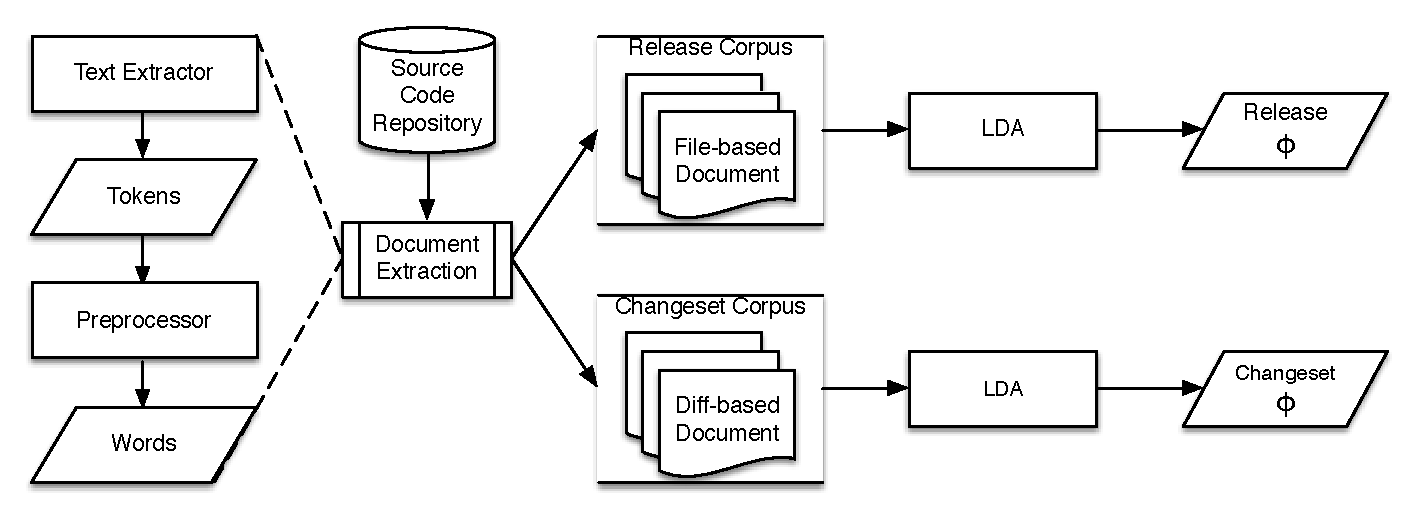
\includegraphics[width=.75\textwidth]{changeset}}
\caption{Source code indexing and modeling process}
\label{fig:process}
\end{figure*}



The source code indexing and modeling process,
as illustrated in Figure~\ref{fig:process},
defines a method for processing text (source code) into
a format suitable for efficient querying of the system, and
producing the result of such a query.
Terminology used in this section will first be defined, followed by an overview of each step of the process.

    \subsubsection{Terminology}
    We use the same terminology as Biggers et al.~\cite{Biggers-etal:2011}.
    They provide the following definitions:
    \begin{itemize}
    \setlength{\itemsep}{1pt}
    \setlength{\parskip}{0pt}
    \setlength{\parsep}{0pt}
    \item \textit{Term}: a sequence of letters and the basic unit of discrete data in a lexicon
    \item \textit{Token}: a sequence of non-whitespace characters; contains one or more terms
    \item \textit{Entity}: a source element such as a class or method
    \item \textit{Identifier}: a token representing the name of an entity
    \item \textit{Comment}: a sequence of tokens delimited by language-specific markers, e.g., /* */
    \item \textit{String literal}: a sequence of tokens delimited by language-specific markers, e.g., “ ”
    \item \textit{Word}: the smallest free form in a language
    \end{itemize}
    Further, a term is described as being one of:
    word, abbreviation of a word, contraction of one or two words,
    or acronym of a series of words.

    \subsubsection{Indexing}
    The indexing process is illustrated on the left side of Figure~\ref{fig:process}.
    It converts source code into a corpus, or collection of documents.
    A document is a collection of terms that appear in a source code entity.
    Each entity in the source code will have an associated document in the resulting corpus.

    Typically, this indexing process has been used on source code files ~\cite{Marcus-etal:2004}.
    Hindle et al.~\cite{Hindle-etal:2009} creates tokens based on the commit log messages.
    This model is similar to ours in that it uses tokens mined from commits rather than source code files.
    Nevertheless, we are unaware of any previous approach to indexing that is similar to what we propose,
    and our investigation of using indexing with LDA is the first of its kind in the software engineering domain.

    \subsubsection{Text Extraction}
    The text extraction stage receives as input source code and produces a list of tokens.
    The text extractor can be configured to tokenize some combination of
    the comments, string literals, and identifiers present in the source code.
    Biggers et al.~\cite{Biggers-etal:2011} evaluate the relative performance of an LDA-based FLT
    given text from different combinations of these sources
    and report that including text from all three sources generally provides the best performance.
    Hence, we choose not to configure a text extractor.
    Instead, we opt for using the entire entity as a whole where applicable.

    \subsubsection{Preprocessing}
    \label{sec:preprocessing}
    The preprocessing stage takes each token produced by the text extractor
    and applies a series of processing steps, producing one or more terms.
    Common steps include~\cite{Marcus-etal:2004, Marcus-Menzies:2010}:
    \begin{itemize}
    \setlength{\itemsep}{1pt}
    \item \textit{Identifier Splitting}:
    divide a token into terms based on common coding conventions
    such as camel case and underscores and on punctuation or other symbols.
    The original term can be kept or discarded.
    \item \textit{Case Normalization}:
    convert all uppercase characters to lowercase, or vice-versa.
    \item \textit{Stop Word Filtering}:
    discard natural language articles (e.g., ‘the’, or ‘a’),
    programming language specific keywords,
    and common words as defined by a stop-list.
    \item \textit{Word length filtering}:
    discard words that do not meet a length requirement (e.g. too short or two long)
    \item \textit{Stemming}:
    strip words of prefixes and suffixes to leave a common root.
    This allows different forms of the same word
    (e.g., ‘stemmer’, ‘stemming’)
    to be conflated to a single term
    (e.g., ‘stem’).
    Biggers and Kraft found that stemming did not improve text retrieval based feature location that used LDA~\cite{Biggers-Kraft:2012}.
    Hence, we chose not to perform stemming.
    \end{itemize}

    \subsubsection{Term Weighting}
    The term weighting step assigns a numeric value, or weight, to each item in the corpus.
    Common term weighting schemes described in the literature are
    binary, term count, term frequency, and
    term frequency-inverse document frequency (tf-idf)~\cite{Salton:1988}.
    Bassett and Kraft discovered that when using LDA-based Feature Location Techniques a weighting of eight for method names and a weighting of one for the method call~\cite{Bassett-Kraft:2013}.
    We chose not to weight terms, giving all terms equal weighting.

    \subsubsection{Model Generation}
    Model generation is depicted in the center of Figure~\ref{fig:process}.
    This stage takes a corpus as input and processes it using a TR method
    to produce a model of the source code as output.
    The TR methods commonly used in this stage include the VSM~\cite{Salton:1971},
    LSI~\cite{Deerwester-etal:1990},
    and LDA~\cite{Blei-etal:2003}.

%Once a model has been generated, further retrieval of information or
%querying may be done, depending on the task. Common tasks in software
%engineering include bug localization, feature location, blah blah 

\subsection{Latent Dirichlet Allocation}

Latent Dirichlet allocation (LDA)~\cite{Blei-etal:2003} is a generative topic model.
LDA models each document in a corpus of discrete data as a finite mixture over a set of topics
and models each topic as an infinite mixture over a set of topic probabilities.
That is, LDA models each document as a probability distribution
indicating the likelihood that it expresses each topic and
models each topic that it infers as a probability distribution
indicating the likelihood of a word from the corpus being assigned to the topic.

Inputs to LDA are:
\begin{itemize}
\setlength{\itemsep}{1pt}
\item $D$, the documents
\item $K$, the number of topics
\item $\alpha$, the Dirichlet hyperparameter for topic proportions
\item $\beta$, the Dirichlet hyperparameter for topic multinomials
\end{itemize}

The documents provided are considered a bag-of-words,
represented as a vector of length $V\!$, the size of the vocabulary.
The original word ordering and grammatical information is discarded.

Outputs of LDA are:
\begin{itemize}
\setlength{\itemsep}{1pt}
\item $\phi$, the term-topic probability distribution
\item $\theta$, the topic-document probability distribution
\end{itemize}

The parameters $\alpha$ and $\beta$ are used to control the smoothing of the model.
Topic distribution per document is influenced by $\alpha$,
and term distribution per topic is influenced by $\beta$.
Decreasing the value of $\alpha$ allows for fewer topics to be associated with a document,
while decreasing the value of $\beta$ generates topics that produce fewer terms
(increasing the number of topics needed to model the corpus).
Decreasing these values makes the computed probability distributions, $\phi$ and $\theta$,
more specific, increasing the decisiveness of the model.

\subsection{Topic Modeling Software}

Feature location as presented by Rajlich et al.\ is a way of locating concepts within code to increase understanding of the program as a whole~\cite{Rajlich-Wilde:2002}.
Linstead et al.\ outlined a statistical model using LDA that was able to mine these concepts from source code~\cite{Linstead-etal:2007b}.
Linstead et al.~\cite{Linstead-etal:2007} used author-topic models to retrieve
developer contribtions from source code.
Lukins et al.~\cite{Lukins-etal:2008} implemented a way of using LDA to locate bugs in source
code that performed better than LSI-based information-retrieval
techniques.
Basset et al.~\cite{Bassett-Kraft:2013} extended this work
and studied various weightings of various terms in source code
to improve LDA-based feature location accuracy in five Java systems.
They found that a multiplier of eight for method names and a multiplier
of one for method calls is best for accuracy.

Hindle et al.\ proposed that topic modeling ought be used on windowed topics~\cite{Hindle-etal:2009}, which were smaller in scope than a larger analysis based on a "global topic analysis" as much of the previous scholarship on topic models in SE used.
The model that Hindle et al.\ used applied LDA to each separate commit's log comments independently then link the topics together in a way that is known as the Link model.
They found that there were certain topics that would not register in a larger analysis but would be important at certain times in the development process.

Thomas et al.\ proposed that the model that ought be used for topic modeling should incorporate only the changes between versions~\cite{Thomas-etal:2011} to better represent the evolution of a corpus over time.
The diff model, as they named it, processes the source code so that all duplicated code is removed, then creates topic models based on the remaining altered source code.
This method created more distinct topics than the previously used models.
The metric that they used to measure the number of distinct topics was topic distinctness (More technical description of TD).
The higher topic distinctness a topic has the more distinct that topic is from other topics.
This is the measure that we will use to compare our model to a model based on releases.

\begin{comment}
Software source code is often compiled through a series of commits that change the source code between releases.
These commits can be of many sizes from a small change in a function to additions of many functions.
The person who commits these changes is seen as being the owner of the code~\cite{Corley-etal:2012}.
The owner of the code is assumed to have a greater working knowledge of the code in question than other members of the design team.
Being able to determine who would know most about a certain topic would allow someone working on a design team to know who is best fit to solve an issue pertaining to a certain topic.
Unfortunately, most of the topic modeling that is currently used to determine ownership is only based off of larger releases rather than intermediate changes.
These types of topic models can be problematic if you are working between releases.
Think for a second that you are a project manager at a software company with a rapidly approaching release deadline.
There is a problem of some sort with the code, and through the use of a topic model you could be able to identify precisely who should be delegated the task of fixing it.
With the type of dynamic topic model like we are proposing, this is easily attainable.
A model based on the change sets between commits would allow software developers never to have an obsolete model.
While there has been some research in the use of commit log comments~\cite{Hindle-etal:2009}, we are not aware of any analyses of topic models that have been created by using the differences of the source code between commits.
\end{comment}
